\documentclass[14pt]{article}

\usepackage[a4paper, margin=.5in]{geometry}

\usepackage{multirow}
\usepackage{multicol}
\usepackage{subcaption}
\usepackage{authblk}
\usepackage{biblatex}
\usepackage{graphicx}
\usepackage{caption}
\usepackage{algpseudocode}
\usepackage{amssymb}
\usepackage{amsmath}
\usepackage{hyperref}
\usepackage[ruled]{algorithm2e}
\usepackage{float}
\graphicspath{{./images/}}

\title{\raggedright{Point Cloud Sampling Network}}
\author[a]{\raggedright{Huang}}
\author[a,*]{\raggedright{Yong Liu}}
\author[a,b]{\raggedright{Jie Liang}}
\affil[a]{\raggedright{Laboratory of Advanced Perception on Robotics and Intelligent Learning, College of Control Science and Engineering, Zhejiang University, Hangzhou, China}}
\affil[b]{\raggedright{Institute of Mechanical and Electrical Engineering, Beijing, China}}
\date{}
\addbibresource{bibliography.bib}




\begin{document}
\maketitle

\section{Abstract}
The increasing number of points in 3D point clouds has brought great challenges for subsequent algorithm efficiencies. Down-sampling algorithms are adopted to simplify the data and accelerate the computation.

\begin{multicols}{2}
\section{Introduction}
Existing works  \cite{qi2017pointnet++,hu2020randla,qi2019deep} often use random sampling and the farthest point sampling (FPS) to down-sample the point clouds.The differences between our work and former learning-based works are presented in \href{fig:fig1}{Fig. 1}.The discrepancy between progress-net and our method is presented in \href{fig:fig1}{Fig. 1}-(b) and (c).

\begin{figure}[H]
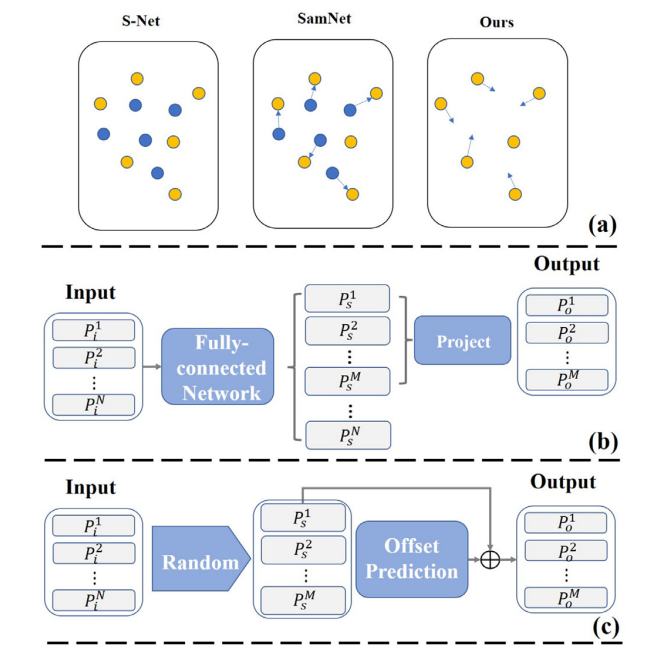
\includegraphics[scale=0.5]{image1}
\caption{(a) shows the differences between learning-based sampling strategies, while (b) and (c) present the discrepancy between progress-net and our method in multiresolution sampling}
\label{fig:fig1}
\end{figure}

Our contributions can be summarized as:
\begin{itemize}
	\item We propose a novel learning-based point cloud sampling
framework named fast sampling network (FPN) by driving existing randomly sampled points to better positions;
    \item We introduce a hybrid training strategy to help FPN adapt to
different sampling resolutions by randomly introducing selecting the resolution of initial points during training;
\end{itemize}

\section{Methodology}
\subsection{Basic Pipeline}
The basic pipeline of FPN is presented in \href{fig:fig2}{Fig. 2}. We aggregate global features from the input points with a set of multilevel perceptions (MLPs) and Max Pooling following PointNet \cite{qi2017pointnet}

\subsection{Hybrid Training Strategy}
The achievement of HTS is presented as \href{alg:1}{Algorithm 9}.
\subsection{Loss function}
The range constraint can be presented as
\begin{equation}
	\mathcal{L}_{rc}=\frac{1}{N}\sum||S_o-S_i||_2
\end{equation}

For reconstructionrelated tasks, it may be Chamfer Distance or Earth Mover Distance [22] defined as\\

\begin{equation}
\begin{split}
	\mathcal{L}_{task}&=L_{CD}(S_1,S_2)\\
	&=\frac{1}{2}\Biggl(\frac{1}{|S_1|}\sum_{x\in S_1} min_{y\in S_2})||x-y||_2+\frac{1}{|S_2|}\sum_{x\in S_2}min_{y\in S_1}||x-y||_2\Biggr)
\end{split}
\end{equation}
or
\begin{equation}
	\mathcal{L}_{task}=\mathcal{L}_{EMD}(S_1,S_2)=min_{\phi ;S_1\rightarrow S_2}\frac{1}{|s_1|}\sum_{x \in S_1}||x-\Phi(x)||_2
\end{equation}

\section{Experiments}
\subsection{Dataset and Implementation Details}
\label{subsec:4.1}
\begin{table}[H]
    \caption{The number of neurons in networks. $f_1 , f_2 , f_3$ are modules in \href{fig:fig2}{Fig. 2}.}
    \begin{tabular}{cccc}
		\hline
    	&$f_1$&$f_2$&$f_3$\\
		\hline
		MLPs&(128,256,256)&(128,256,256)&(128,128,3)\\
		\hline
    \end{tabular}
	\label{table:1}
\end{table}

\begin{table}[H]
    \caption{The comparison on optimal clustering.}
    \begin{tabular}{ccccc}
		\hline
    	Center&Iterations&1&10&100\\
		\hline
		16&FPS&2.43&2.00&1.98\\
		&Ours&2.16&1.98&1.96\\
		32&FPS&1.20&1.02&1.00\\
		&Ours&1.11&1.00&1.00\\
		\hline
    \end{tabular}
	\label{table:2}
\end{table}
The hyper-parameter $\lambda$ is tuned on the validation split of ShapeNet.Detailed network structures are shown in \href{table:1}{Table 1}

\subsection{Discussion and Clustering}
Except down-stream tasks such as reconstruction or recognition, down-sampled points can also be adopted as the initial clustering centers.  The results are presented in \href{table:2}{Table 2}.

\begin{figure*}
  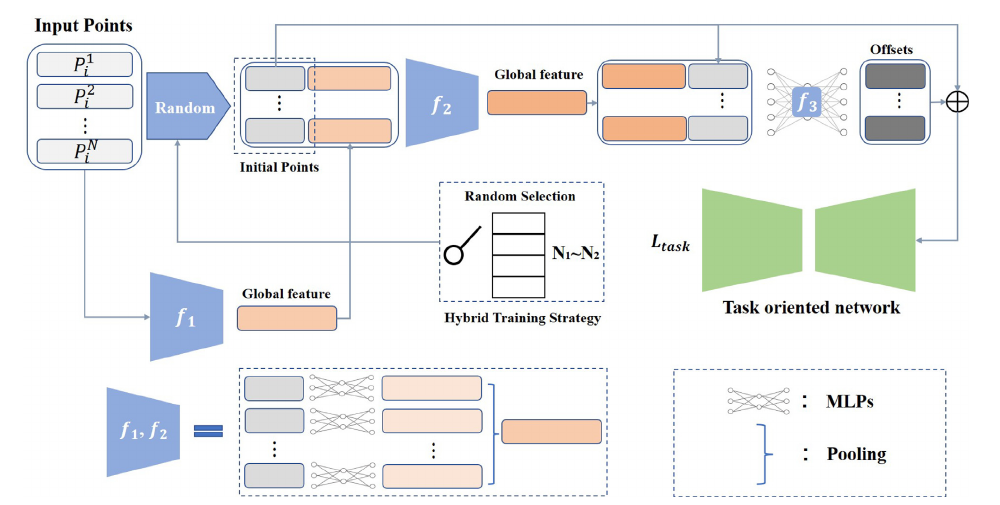
\includegraphics[width=\linewidth]{image2.png}
  \caption{The whole pipeline of FPN. The + denotes element-wised addition. $f_1$ and $f_2$ aggregate features by MultiLayer Perceptrons(MLPs) and pooling, while $f_3$ is a group of MLPs to predict offsets from coordinates and features. The task network is corresponding to the specific task, such as point cloud recognition and reconstruction. $L_{task}$ is the loss constrained the task network.}
 \label{fig:fig2}
\end{figure*}

\subsection{Ablation Study}
\textbf{The influence of range constraint.} Note that this is only conducted to observe the influence of range constraint weight $\lambda$ on sampling performances instead of the tuning of $\lambda$, which is chosen according to the val set introduced in \href{subsec:4.1}{Section 4.1}.

\begin{algorithm}[H]
 \label{alg:1}
 \caption{Training with Hybrid Training Strategy}
 \SetAlgoNoLine
 \KwIn{data $X$, the number of iterations $iter$, the number of resolutions $m$;}
 $prob_1, prob_2, \ldots, prob_m = \frac{1}{m}, \frac{1}{m}, \ldots, \frac{1}{m};$\\
 \SetKwFor{For}{for}{do}{end for}
 \For{$i=1$ \KwTo $iter$}
 {
 Select the resolution $r$ according to $prob_1,\ldots, prob_m$;\\Train FPN by descending gradient:$\Delta_{\theta_{FPN}}\mathcal{L}_{loss}\left(Y_{X, r}\right)$\\
 }
\end{algorithm}

\printbibliography
\end{multicols}

\end{document}
